%!TEX root = ../main.tex

\chapter{Preliminaries\label{chap:preliminaries}}

\section{Radioactivity}
Radioactivity is a natural phenomenon in which unstable atomic nuclei undergo spontaneous decay, emitting radiation in the form of particles or electromagnetic waves. 
This process occurs in certain types of atoms, known as radioactive isotopes or radionuclides. 
A radioactive atom attempts to reach stability by releasing energy in form of ionizing radiation.
Ionizing radiation refers to any form of radiation with enough energy to remove tightly bound electrons from the orbit of an atom.
Among others, radioactive decay releases three main types of ionizing radiation: alpha particles, beta particles, and gamma rays. 


\section{Properties of ionizing radiation}
\subsection{Activity}% %%{
"Activity" is one of the terms used to quantify and describe properties of radioactive sources.
It is defined as number of radioactive decays per second.
The unit of activity is called Becquerel ($\si{\becquerel}$) and belongs to SI\footnote{International System of units} units.
In other words, if a radioactive source has activity one Becquerel, it means that one unstable nucleous decays per second (on average, since the decay is a stochastic process).
It is important to note that the Becquerel only measures the rate of decay and does not take into account the type or energy of the radiation involved.% %%}

  \subsection{Inverse square law}% %%{
The inverse square law is a fundamental principle that applies to diverse physical phenomena including radiation.
It describes how the intensity of radiation decreases with increasing distance from the source.
The intensity of radiation is inversely proportional to the square distance from the source:
\begin{equation}
  intensity \approx \frac{1}{distance^2}.
\end{equation}
For example doubling the distance to the source means that the intensity decreases to $\frac{1}{4}$.
As illustrated in figure \ref{fig:islaw}, this principle comes from the fact that the radiation spreads out over larger area when the observer is further away from the source.
This rapid decrease makes the search for sources of ionizing radiation challenging since it limits the sensing range of the detectors.

  \begin{figure}[!h]
    \centering
      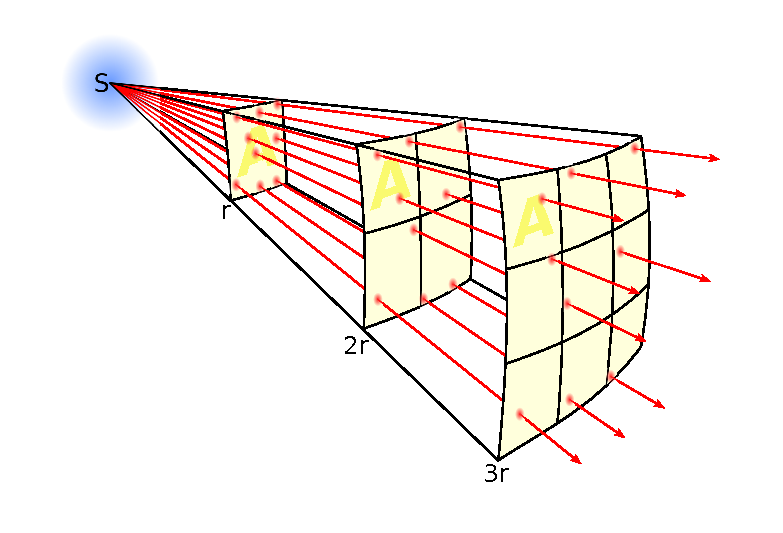
\includegraphics[width=0.5\textwidth]{./fig/photos/Inverse_square_law.eps}
    \caption{An illustration of inverse square law for radiation.\ Source: By Borb, CC BY-SA 3.0, \url{https://commons.wikimedia.org/w/index.php?curid=3816716i}}
      \label{fig:islaw}
  \end{figure}

% %%}

\subsection{Health risk}% %%{
Several health risks are associated with ionizing radiation.
While traversing the human body, ionizing radiation can interact with living tissues causing damage or mutations of individual cells.
In long-term horizon, exposure to ionizing radiation might cause cancer or even genetic disorders.
The severity of health problems depend on exposure time and dose of absorbed radiation.
High doses of ionizing radiation over a short period can cause disease named acute radiation syndrome (radiation sickness).
The disease is manifested by nausea, vomiting, fatigue or even skin burns. 
Depending on the absorbed radioactive dose, it causes several neurological or cardiovascular problems or might lead to death.% %%}






\section{Main types of ionizing radiation}
\subsubsection{Alpha radiation}
Alpha radiation is an emission of positively charged alpha particles consisting of two protons and two neutrons bound together (helium nuclei).
This gives alpha particles a significantly larger mass and higher reactivity compared to other types of ionizing radiation.
On the other hand, they interacts strongly with matter and can't penetrate far.
Alpha particles can travel only few centimeters in air and can be blocked by single sheet of paper or outer layer of human skin.
Because of that, external sources of alpha radiation are generally not considered a significant threat to human health.
The limited range of alpha radiation makes it difficult for sensing from distance.

\subsubsection{Beta radiation}
Beta particles are high-energy, high-speed electrons or positrons.
Due to their smaller size and weaker electrical charge, they are generally more penetrating and less reactive than alpha particles and can reach further in materials.
Several centimeters thick sheet of aluminium or plastic is typically sufficient to block the beta radiation.
In terms of travel through the air, beta particles have range of few meters.
Although the beta radiation is generally less dangerous than gamma, when particles come into contact with human skin, they can penetrate the outer layers and cause skin burns as the particles disrupt cellular processes.

\subsubsection{Gamma radiation}
Gamma rays are often produced alongside alpha or beta particles during radioactive decay. 
Unlike them, gamma radiation of composed of high energy photons. 
They are extremely penetrating and can travel long distances in air as well as get through most of materials or living tissues thanks to their high energy and lack of charge.
Only thick layer of concrete or lead might block this type of ionizing radiation.
These features make the gamma radiation significantly more dangerous than alpha and beta.
The long range of gamma radiation together with negative effects on human health makes it ideal candidate for remote sensing and detection.

  \begin{figure}[!h]
    \centering
      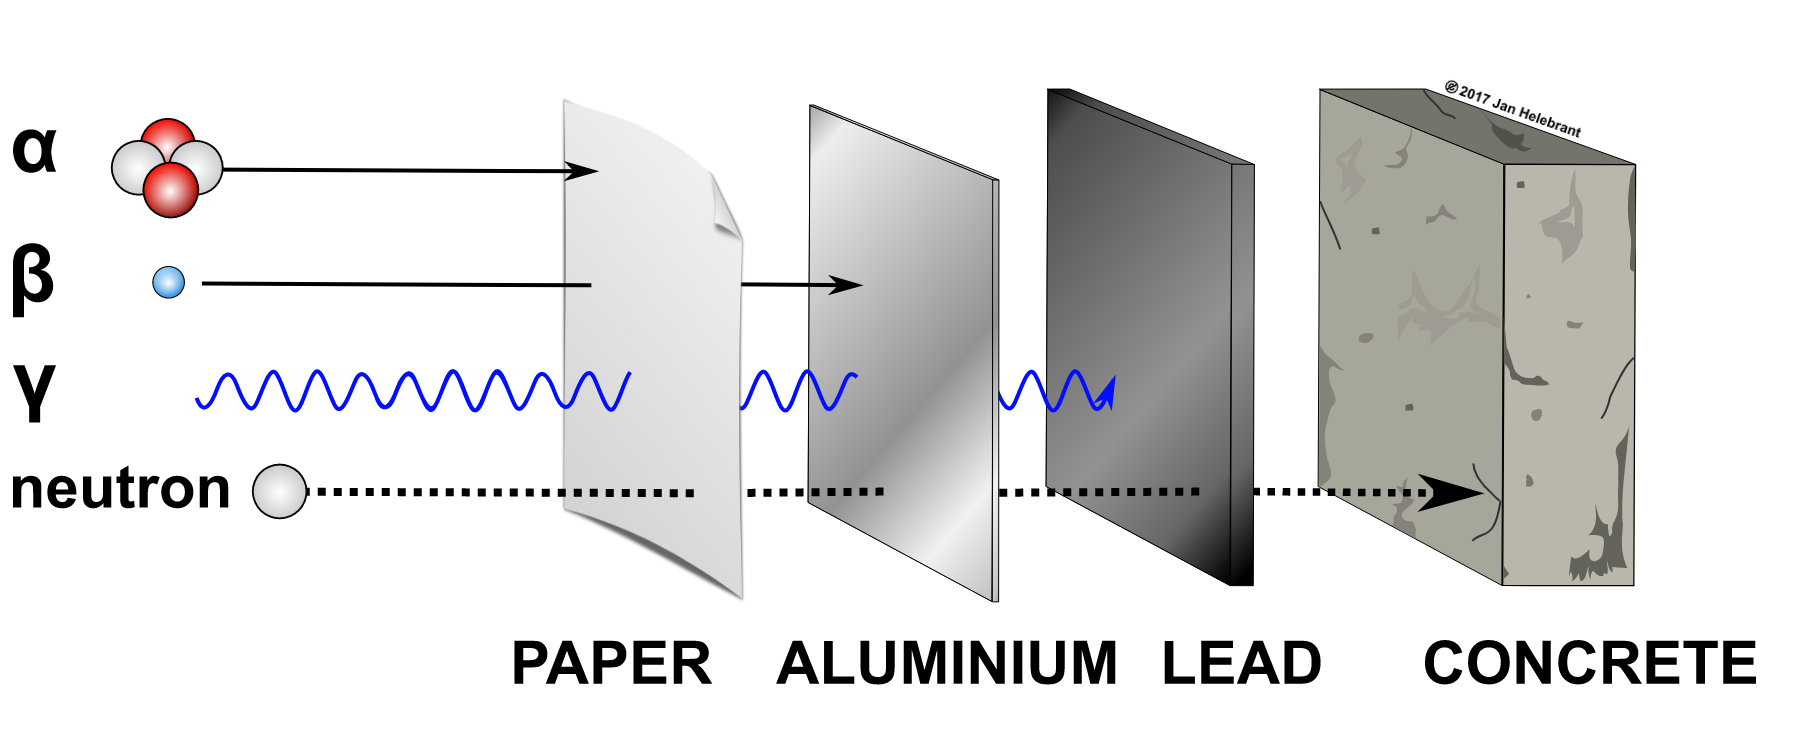
\includegraphics[width=0.6\textwidth]{./fig/photos/pene2.png}
    \caption{Penetrating power of different types of radiation. Source:\url{https://openclipart.org/detail/274074/penetrating-power-of-different-types-of-radiation-alpha-beta-gamma-and-neutrons}}
      %\label{fig:islaw}
  \end{figure}


%On the other hand, ionizing radiation might also have positive impacts on human health.
%It is used in medicine for both diagnostic and therapeutic purposes.

\section{Interaction of $\gamma$ radiation with matter}
Sensing of $\gamma$ radiation is possible through interactions of ionizing photons with imaging devices.
Several interactions might occur when high energetic photon travels through matter, depending on the energy of the incoming photon as well as on the properties of material.
Three main types of interactions are: photoelectric effect, compton scattering and pair production.
The figure \ref{fig:dominant} describes the dominant type of interations depending on the energy of incoming photon and atomic number of the material.

\begin{figure}[!h]
  \centering 

    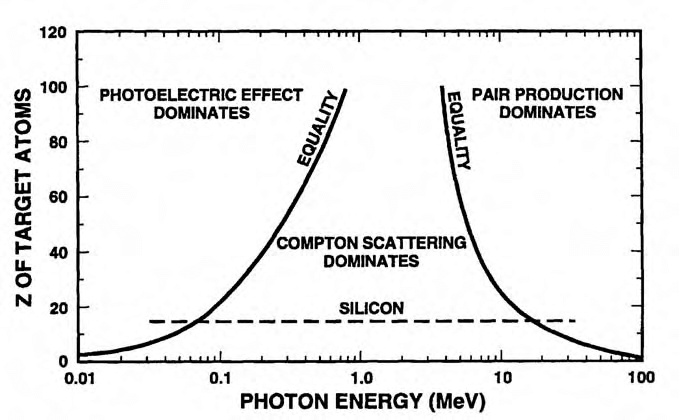
\includegraphics[width=0.6\textwidth]{./fig/photos/dominant.png}
  \caption{Dominant types of interactions for different energy of photon (x-axis) and atomic number of matrial (y-axis). Source of image: \cite{schwank}}
    \label{fig:dominant}
  
\end{figure}

\subsection{Photoelectric effect and pair production}
In \ac{PE}, also reffered as photoelectric absorbtion, the $\gamma$ photon interacts with orbital electron of absorbing atom.
The photon transfers all its energy to the electron and disappears.
As a consequence, the electron exceeds its binning energy and is emitted from the atom.
The photoelectric absorption is dominant at lower energies of incident photon, however it may occur at any photon energy.
The \ac{PP} occurs only if the $\gamma$ photon has energy exceeding $\approx \SI{1}{\mega\electronvolt}$.
Such very high energetic photon interacts with the nucleolus of the atom.
An electron-positron pair is created as a result of the interaction.

\subsection{Compton scattering}
Third possible interaction (predominant on mid-level energies) is the Compton scattering.
During the Compton scattering, the $\gamma$ photon interacts with an electron loosely bound to the nucleus.
The photon with initial energy $E_{0}$ transfers part of it to the electron.
As a result of the interaction, the lower energetic photon with energy $E_{2}$ is scattered and emitted in direction changed by angle $\beta$. 
The energy difference $E_{1} = E_{0} - E_{2}$ is transferred to a bi-product of the interaction - an electron.
The situation is illustrated in figure \ref{fig:scattering}.

\begin{figure}[!h]
    \centering
    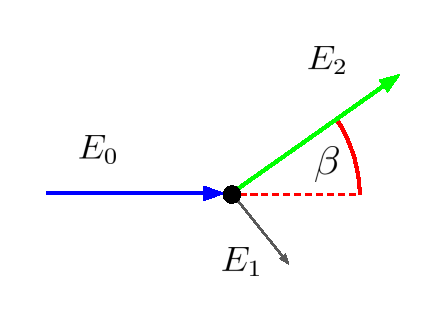
\includegraphics[width=0.3\textwidth]{./fig/photos/compton_simple.eps}
    \caption{An illustration of the Compton scattering. The incident $\gamma$ photon with energy $E_{0}$ (blue) undergoes the Compton scattering. As a result of the interaction, the lower energetic photon (green) with energy $E_{2}$ is emitted under angle $\beta$. Part of the energy ($E_{1}$) is transferred to a bi-product of the interaction- the electron (grey).}
    \label{fig:scattering}
\end{figure}

According to Compton \cite{compton}, the relation of particle energies and scattering angle $\beta$ can be expressed as:

\begin{equation}
E_{2} = \frac{E_{0}}{  1 + (E_{0} / m_{e}c^{2}) (1 - \mathrm{cos} \beta)},
\end{equation}
where $E_{0}$ is the initial energy of the incoming photon, $E_{2}$ is the energy of scattered photon,  $m_{e}$ is the electron rest mass and $c$ is the speed of light in vacuum. 
\mycomment{ %klein nishina % %%{
  The probability that a photon with an energy $E_{0}$ undergoes a Compton scattering through an angle $\beta$ is described by the Klein-Nishina formula
  \begin{equation}
    K(\beta, E_{0}) = \frac{r_{e}^{2}}{2} \left( \frac{E_{2}}{E_{0}}  \right)^{2} \left(  \frac{E_{2}}{E_{0}} + \frac{E_{0}}{E_{2}} - \mathrm{sin}^{2}(\beta)  \right),
    \label{eq:klein_nishina}
  \end{equation}
  where $r_{e}$ is the classical electron radius. 
}% %%}




\section{Measuring radioactivity}
Ionizing radiation is unperceivable by human senses, yet poses a significant health risk for human beings.
Effective monitoring methods are needed to detect and measure a presence of such radiation that is potentially harmful to human beings.
Sensors of ionizing radiation are made of different materials that interact with incoming particles.
Three types of sensors are listed for illustration.
\textbf{Geiger-Müller  counters} are gas-filled tubes, in which the gas is ionized by the passing particles, conducting an electrical charge that can be measured.
\textbf{Scintillation detectors} use a scintillating material that emits light when struck by ionizing radiation.
A photodiode then converts the light to an electrical signal.
Another group of detectors is based on \textbf{semiconductive materials} that are sensitive to ionizing photons. 
The electrons ejected by ionization can be measured and the type and energy of the incoming radiation might be deduced. 

Most of the sensors are simply counting the number of recorded particles and estimates the intensity of particle flux at the given position. 
However, it does not give any information about the direction of incoming particles.
Accurate estimation of distribution of radioactive sources then requires high number of measurements at different positions. 

Following \cite{baca2019timepix}, the direction of incoming particles can be deduced by different detector configurations illustrated in figure \ref{fig:sensor_overview}.
\textbf{Pinhole camera aperture} restricts the field of view by shielding particles from directions other than one narrow passage in the shielding material.
\textbf{Colimators} (frequently used in medical imaging) also restricts the set of possible directions by absorptive material. 
Each part of the detector is responsible for measuring particles coming from certain direction. 
\textbf{Stacked detectors} employ multiple layers, where the particle's direction is computed from interactions at different levels.
Finally, the \textbf{Compton camera} use the Compton scattering for deducing the set of possible directions of the original particle. 




\begin{figure}[!h]
    \centering
    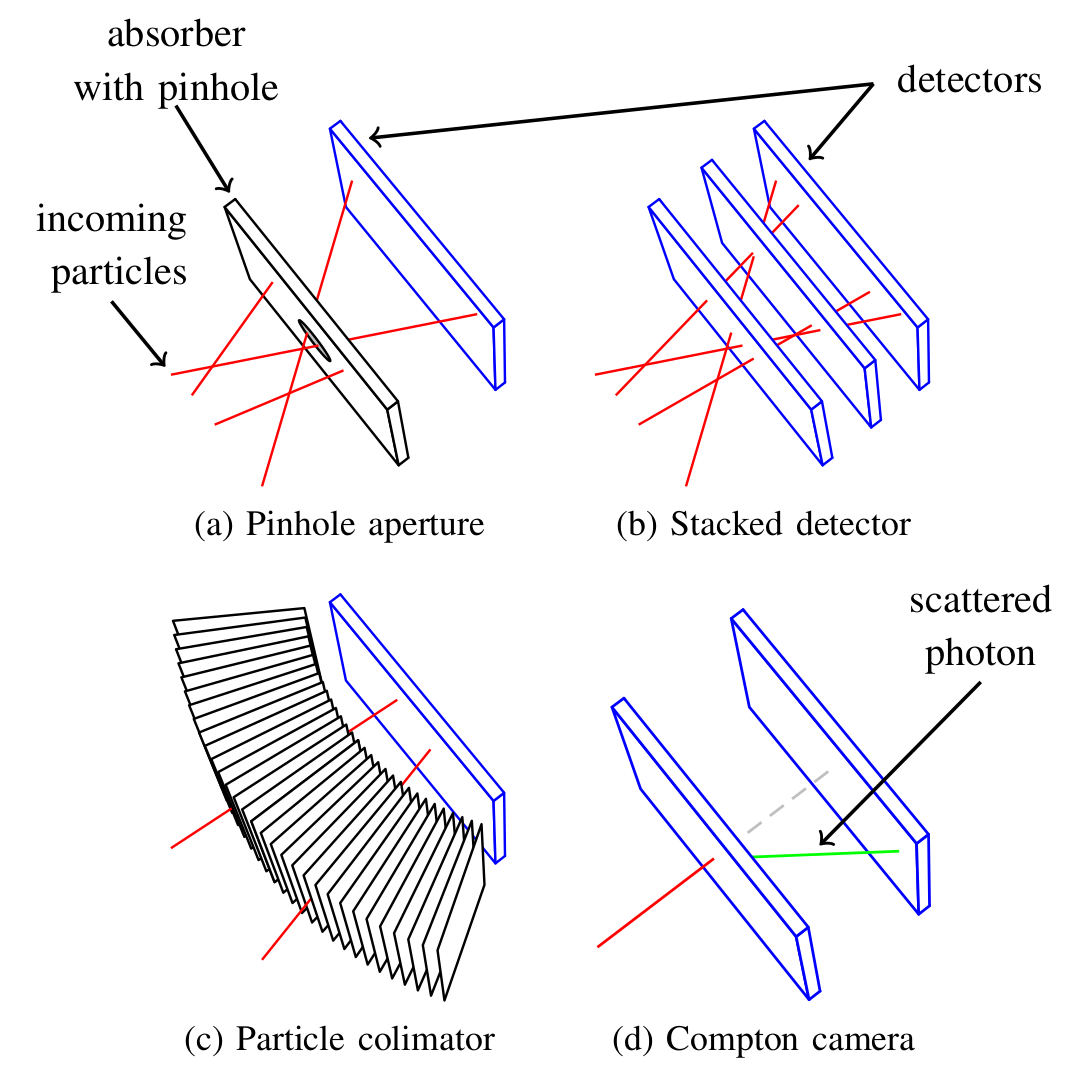
\includegraphics[width=0.5\textwidth]{./fig/photos/detector_overview_baca2019.png}
    \caption{Different ways how to deduce the direction of the incoming particle. Source: \cite{baca2019timepix}}
    \label{fig:sensor_overview}
\end{figure}


\mycomment{
\begin{figure}[!h]% %%{
  \centering
  \subfloat[\centering different ways how to detect the direction of incoming particle. Source: \cite{baca2019timepix}] {
    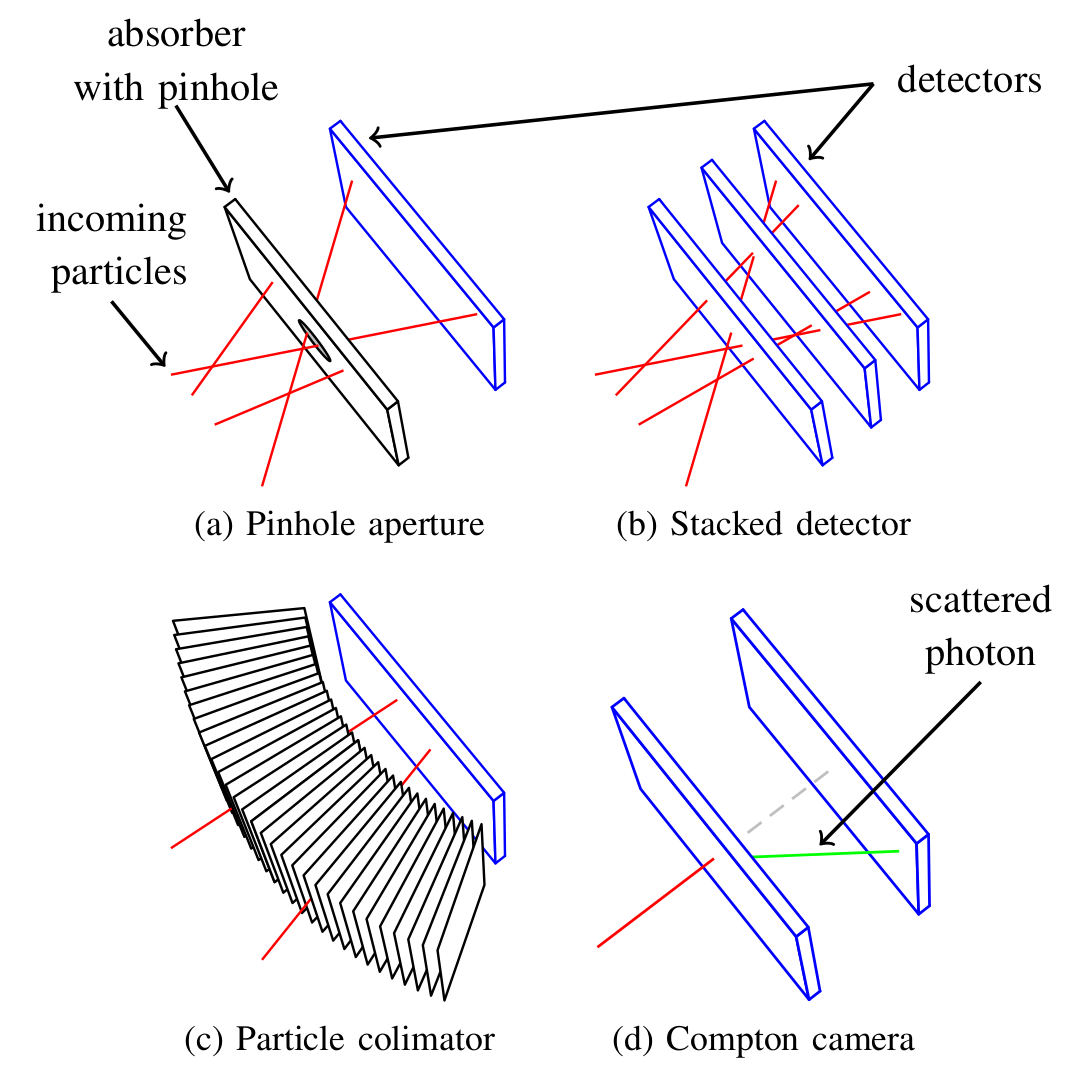
\includegraphics[width=0.49\textwidth]{./fig/photos/detector_overview_baca2019.png}
    \label{fig:sensor_overview}
  }
  \subfloat[\centering Geometry for two-layer Compton camera. The $\gamma$ particle emitted at position $j$ interacts with the first layer of the sensor (scatterer) at position $X_{1}$. A lower energetic photon is scattered under angle $\beta$ and absorbed by the second layer of the detector (absorber) at position $X_{2}$. The reconstructed Compton cone is parametrized by angle $\beta$, axis vector $a$ and origin of the cone $X_{1}$.] {
      \label{fig:compton_camera_geometry}
  
      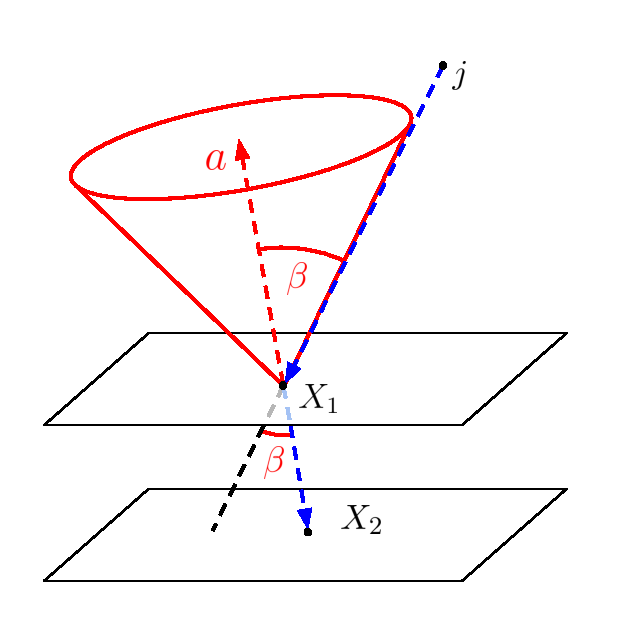
\includegraphics[width=0.49\textwidth]{./fig/photos/compton_camera_modelll.eps}
  }
  \caption{TODO}
  \label{fig:xxx}
\end{figure}% %%}
}


\subsection{Compton Camera}% %%{
The Compton camera is typically composed of two detectors: scatterer and absorber.
The incident photon with energy $E_{0}$ first interacts with the scatterer at position $X_{1}$ in form of Compton scattering.
A bi-product of the interaction (electron with energy $E_{1}$) is immediately captured by the scatterer and its position $X_{1}$ and energy are recorded.
As a result of the interaction, lower energetic photon with energy $E_{2}$ is scattered under (Compton) angle $\beta$.
The scattered photon then interacts in form of \ac{PE} with the absorber.
The absorbed energy $E_{2}$ and the position of the interaction $X_{2}$ are measured and recorded.

The scattering angle $\beta$ can be reconstructed (following \cite{baca2021gamma}) as:
\begin{equation}
  %\beta = \mathrm{arccos} \left (  1-\frac{m_{e}c^{2}E_{2}}{E_{0} (E_{0} - E_{2})} \right )
  \beta = \mathrm{cos}^{-1} 
  \underset{B}{\underbrace{
  \left ( 1+m_{e}c^{2} \left( \frac{1}{E_{1}+E_{0}} - \frac{1}{E_{0}}\right )  \right )
  }},
    \label{eq:compton_beta_formula}
\end{equation}
assuming that $0<B<1$.
Since the Compton scattering is a symmetrical phenomena,  the set of possible directions of incoming particle forms a surface of a cone.
Such conical surface (denoted as Compton cone) is parametrized by the cone axis $a$ (which is a straight line connecting the positions of intersections $X_{1}$ and $X_{2}$), Compton scattering angle $\beta$ and origin of the cone $X_{1}$.
The geometry is illustrated in figure \ref{fig:compton_camera_geometry}.


\begin{figure}[!h]
  \centering
    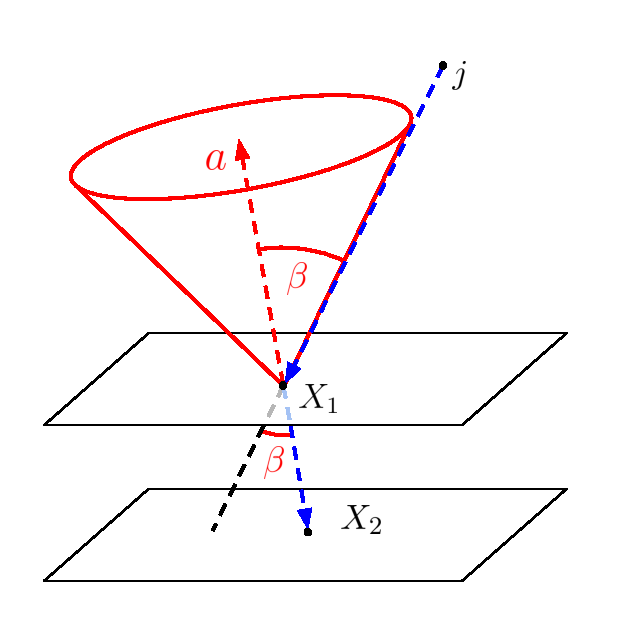
\includegraphics[width=0.4\textwidth]{./fig/photos/compton_camera_modelll.eps}
    \caption{Geometry for two-layer Compton camera. The $\gamma$ particle emitted at position $j$ interacts with the first layer of the sensor (scatterer) at position $X_{1}$. A lower energetic photon is scattered under angle $\beta$ and absorbed by the second layer of the detector (absorber) at position $X_{2}$. The reconstructed Compton cone is parametrized by angle $\beta$, axis vector $a$ and origin of the cone $X_{1}$.}
    \label{fig:compton_camera_geometry}
\end{figure}
% %%}


\section{The MiniPIX TPX3 detector} % %%{
The MiniPIX TPX3 detector\footnote{produced by \textit{Advacam}, https://advacam.com/camera/minipix-tpx3} is a miniature version Timepix3 detector \cite{timepix3}.
It belongs to the class of semiconductor pixel detectors.
The body of the \ac{pix} sensor is made of a compact block of Cadmium telluride (CdTe) semiconductor material with dimensions $14 \times 14 \times 2 \ \si{\milli\meter}$.
Although it has only one detection layer, it can be still used as a Compton camera.

As described in \cite{baca2021gamma} and \cite{baca2019timepix}, the incoming ionizing radiation interacts with the matter of the sensor and separates electrons from the CdTe material.
The newly created electrons are accelerated by a $\SI{450}{\volt}$ electric potential towards one facet of the sensor, where Timepix3 pixel detector is located.
The resolution of pixel detector is $256 \times 256\ \mathrm{px}$, each pixel being $55\ \si{\micro\meter}$ large.
The pixel detector can deduce the energy as well as the type of the absorbed ionizing particle.
Given the measured times of arrival, the coinciding products of Compton scattering might be paired together.
The figure \ref{fig:minipix} depicts the geometry of the \ac{pix} sensor.
The 2D coordinates $\mathbf{\hat{c}}_{x}$,$\mathbf{\hat{c}}_{x}$ (see figure \ref{fig:minipix}) of the interaction are determined by the position of corresponding pixels
The $\mathbf{\hat{c}}_{z}$ coordinate (the depth of interaction in the CdTe block) is unknown.
However, the relative depth position of two coinciding events might be deduced from the times of arrival of the two interactions were captured by the pixel detector.
Because of that, the \ac{pix} detector might be used as a Compton camera.
More technical details related to the sensor operation are provided in \cite{baca2019timepix}.

The \ac{pix} detector has multiple advantages.
It is very compact and lightweight (the size of the whole \ac{pix} sensor is only $80 \times 21 \times 14 \ \si{\milli\meter}$ and it weights $\SI{44}{\gram}$), therefore it can be carried onboard a small \ac{UAV}.
It can report the recorded intersections almost in real time, which allows the to use it for an active strategy, where autonomous \ac{UAV}s react according to the measurements acquired during the flight.

\begin{figure}[!h]
    \centering
  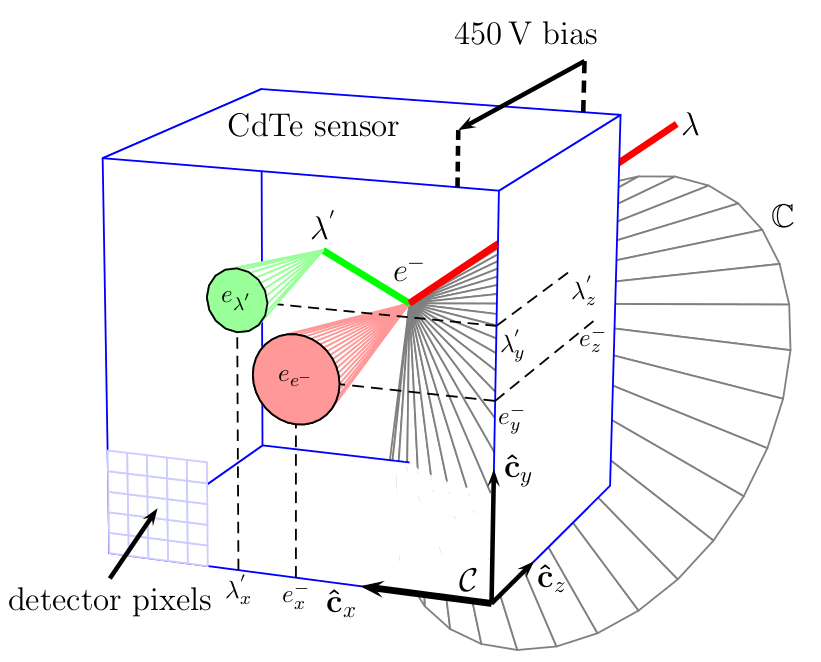
\includegraphics[width=0.5\textwidth]{./fig/photos/minipix.png}
    \caption{An illustration of the detection process inside the MiniPIX TPX3 sensor. Source: \cite{baca2021gamma}}
    \label{fig:minipix}
\end{figure}

\begin{figure}[!h]
    \centering
    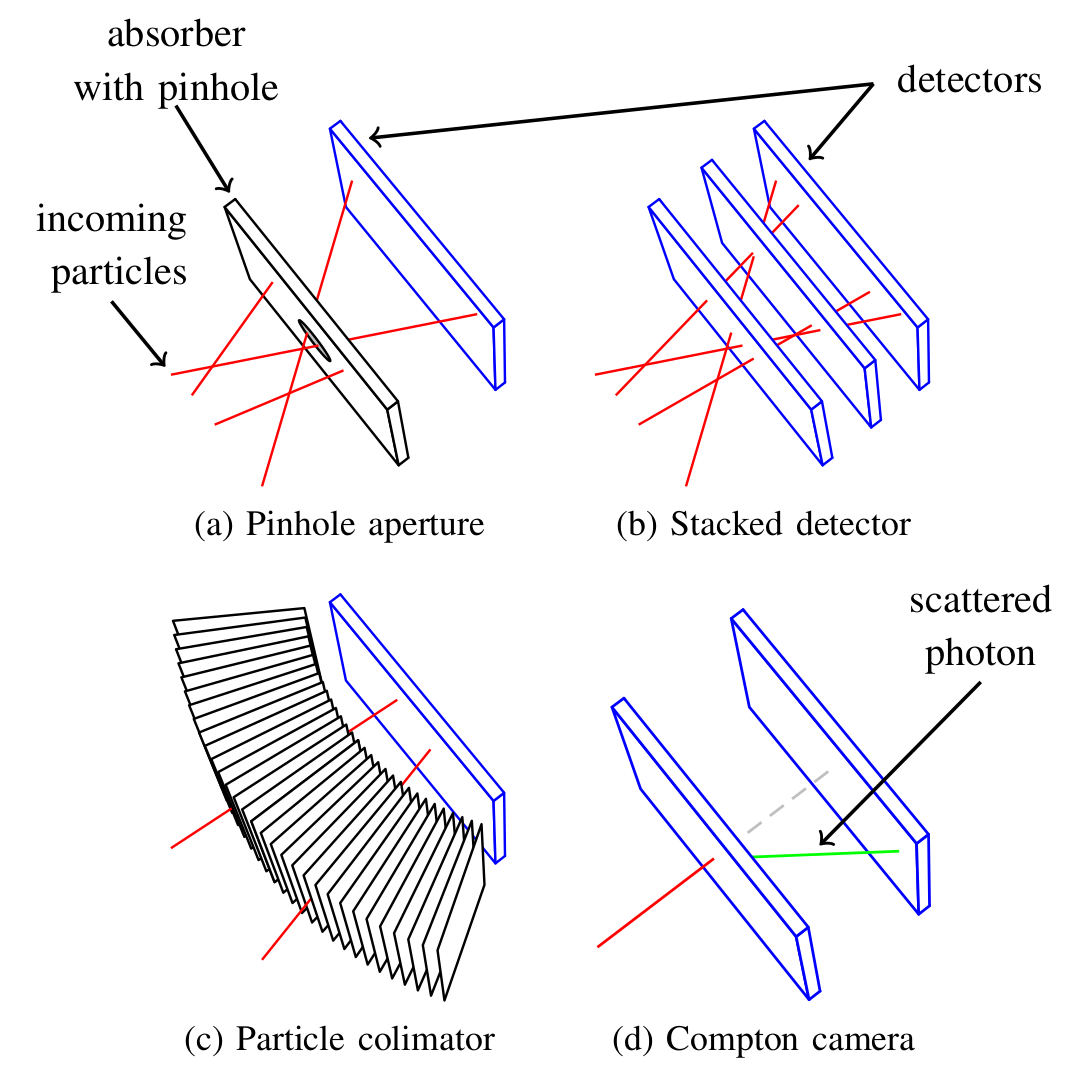
\includegraphics[width=0.5\textwidth]{./fig/photos/detector_overview_baca2019.png}
    \caption{different ways how to detect the direction of incoming particle. Source: \cite{baca2019timepix}}
    \label{fig:sensor_overview}
\end{figure}
% %%}



\section{Robot operating system}

\ac{ROS} is a middleware software framework for robotics applications and research.
It follows a distributed architecture with a peer-to-peer communication model.
Individual software modules (called nodes) can exchange data through standardized messages and services.
The communication between \ac{ROS} nodes is maintained by a central authority called \ac{ROS} master.
The \ac{ROS} master provides the registration of the individual \ac{ROS} nodes as well as maintains communication between them.

\subsubsection{ROS messages and topics}
The fundamental \ac{ROS} communication mechanism used for exchanging messages between different \ac{ROS} nodes is called topics.
Topics are based on a publish-subscribe model, where nodes can either publish data to a topic or subscribe to receive data from a topic. 
Each topic has a specific data type associated with it.
Nodes can publish messages of that data type to the topic, and any subscribed nodes will receive those messages.
Topics enable asynchronous communication between different parts of the robotic system, such as data exchange between sensors and onboard computer.

Another important \ac{ROS} communication concept is called service.
\ac{ROS} services allow nodes to make requests and receive responses to them.
Unlike in \ac{ROS} topics, services provides synchronous request-response communication model.
The client node sends its request to a specific service provided by the server node.
The server node processes the request and generates a response message, which is sent back to the sender.
Such communication scheme might be used for example for triggering some action, requesting path from the planning node and generally in any situation where response from the server node is required.

\section{MRS UAV system}
The MRS UAV system \footnote{available at: \url{https://github.com/ctu-mrs/mrs_uav_system}} \cite{mrs_system} is a research-oriented software platform developed at Czech Technical University in Prague.
The consists of the full control pipeline, including state estimation, sensor fusion, trajectory generation, multirobot communication, planning and feedback control.
It enables operations of groups of autonomous \ac{UAV}s in both indoor and outdoor environments.

    
\subsection{Rosbag}
\subsection{architecture}
\subsection{Nodes, Messages and Services}

%%%%%%%%%%%%%%%%%%%%%%%%
%%%%%%%%%%%%%%%%%%%%%%%%%%
%%%%%%%%%%%%%%%%%%%%%%%
%%%%%%%%%%%%%%%%%%%%%%%%%%%%
%%%%%%%%%%%%%%%%%%%%%%%%%%
%%%%%%%%%%%%%%%%%%%%%%%%


\begin{figure}[!h]% %%{
  \centering
  \subfloat[\centering Cross-section for photon interactions in Silicon in the MeV range. The four dominating interaction mechanisms are photo effect, Compton scattering, pair creation and Rayleigh scattering. Source: \cite{zoglauer}] {
    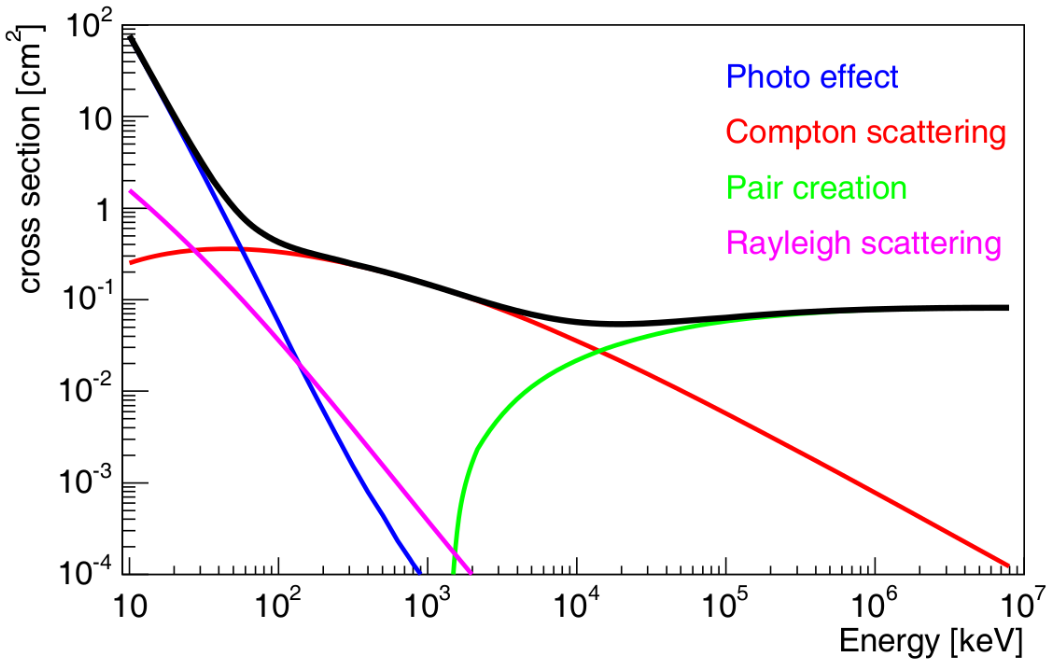
\includegraphics[width=0.2\textwidth]{./fig/photos/cross_stat.png}
    \label{fig:aaaaaa}
  }
  \subfloat[\centering Cross section for compton scattering. Source: \cite{zoglauer}] {

    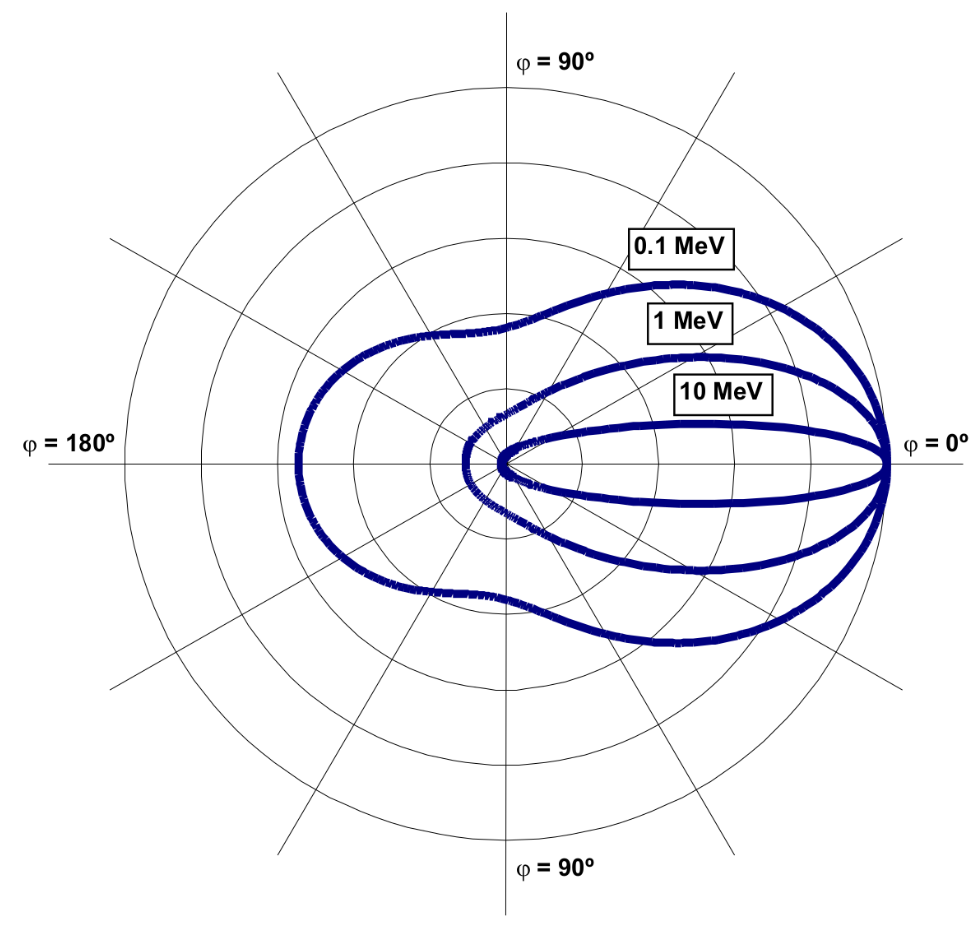
\includegraphics[width=0.2\textwidth]{./fig/photos/cross_section.png}
    \label{fig:aaaaaa}
  }
  \caption{TODO}
  \label{fig:xxx}
\end{figure}% %%}



\alerterror{Old}% %%{
\mycomment{
  \section{Radioactive decay}
  Radioactive decay is a process where an unstable atomic nucleus transforms into a lower-energy state.
  During this process, it loses energy by radiation.
  There are three main types of such radiation - alpha, beta and gamma.
  Whereas alpha particles can be stopped by a sheet of paper and beta particles by aluminium shielding, gamma particles can be blocked only using a thick block of lead or a massive concrete wall.
  Moreover, highly energetic gamma rays have a negative effect on the human body, causing damage on a cellular level.
  Being exposed to such radiation poses a risk of severe health problems or death.

  \section{Some properties of $\gamma$ radiation}
  \subsection{Inverse square law}
  \subsection{Interaction with matter}

  The quantity of emitted particles ("strength" of the source) is expressed in Becquerels.
  It is a SI unit defined as the number of emitted particles per second.

  \section{Interaction with matter}
  As the gamma particle passes through matter, there are three possible effects that might happen:
  \textbf{the photoelectric effect}, \textbf{Compton scattering} and \textbf{pair production}.

  \textbf{The photoelectric effect} is typical at low energies of gamma rays. A photon undergoes an interaction with an electron that is bound in an atom. The incident photon completely disappears in this interaction. A product of this interaction is a photon.
  \textbf{The Compton effect} is typical for mid-energetic gamma rays. In this process, an incident gamma photon loses energy to an atomic electron. A new lower energetic photon is emitted in a different direction (hence the frequently used term "Compton scattering").
  \textbf{Pair production} is typical for high-energetic gamma rays. It is a process in which a photon of sufficient energy is converted into an electron and a positron.

  The Compton effect (published in 1923 \cite{}) describes the way how a (gamma or X-ray) photon interacts with a static electron. An incident photon with wavelength $\lambda$ losses some energy to the electron. A new lower energetic photon with wavelength $\lambda^{\prime}$ is emitted under angle $\beta$. Thanks to the law of conservation of energy and momentum, Compton derived the following equation
  \begin{equation}
      \lambda^{\prime} = \lambda + \frac{h}{m_{e}c}(1-\mathrm{cos} \beta),
  \end{equation}
  where $\lambda$ is the wavelength of the incident photon, $\lambda^{\prime}$ is the wavelength of the emitted photon, $h$ is the Planck constant, $m_{e}$ is the electron rest mass, $c$ is the speed of light and $\beta$ is the scattering angle.

  \begin{figure}[!h]
      \centering
      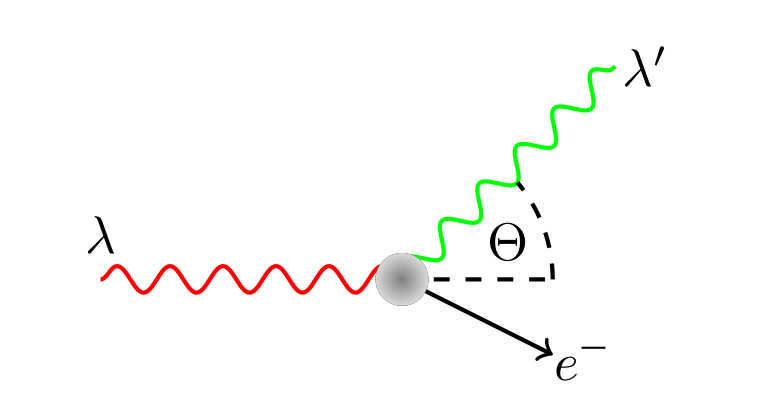
\includegraphics[width=0.3\textwidth]{./fig/photos/scattering.png}
      %\label{fig:scattering}
      %\caption{An illustration of Compton scattering. The incident photon interacts with the static electron. As a result, a new lower energetic photon is emitted in a direction changed by $\beta$ as part of its energy is transferred to electron $e^{-}$. Source: \cite{baca2021gamma}}
  \end{figure}


  \subsection{Klein Nishina formula}
  TODO

  \subsection{Compton effect}
  TODO


  \section{Compton camera}
  This effect is the fundamental principle in a sensor called a Compton camera. 
  The sensor is typically composed of two main components: the scatterer and the absorber. 
  The incident photon first interacts with the scatterer, where the lower energetic photon is emitted under angle $\beta$ (thanks to the Compton effect). 
  Since it is more common to measure energies instead of wavelength, we can rewrite the Compton formula as
  \begin{equation}
  E_{\lambda^{\prime}} = \frac{E_{\lambda}}{  1 + (E_{\lambda} / m_{e}c^{2}) (1 - \mathrm{cos} \beta)},
  \end{equation}
  where $E_{\lambda}$ is the energy of the incoming photon from the source, $E_{\lambda^{\prime}}$ is the energy of the scattered photon.  
  The bi-product of the interaction (electron $e_{e^{-}}$) is immediately measured in the scatterer, and its position is recorded.
  Then, the scattered lower energetic photon interacts with the second layer of the sensor - the absorber. 
  The photoelectric effect is witnessed while measuring the product of it - the energy of the electron $e_{\lambda^{prime}}$ and its position on the absorber.

  Now we can express the scattering angle $\beta$ as
  \begin{equation}
      \beta = \mathrm{arccos} \left (  1-\frac{m_{e}c^{2}E_{\lambda^{\prime}}}{E_{\lambda} (E_{\lambda} - E_{\lambda^{\prime}})} \right )
      %\label{eq:compton_beta_formula}
  \end{equation}

  Given the measurements on the scatterer and absorber and computed scattering angle $\beta$ using the equation \ref{eq:theta} (using known energy of the incoming photon $E_{\lambda}$), we can reconstruct a set of possible directions from where the original photon arrived. Since the Compton effect is symmetrical, the set of possible directions towards the source of ionizing radiation forms a surface of a cone.



  \subsection{MiniPIX TPX3 sensor}
  The sensor used in this work is a small CdTe event-based camera that is capable of witnessing the interactions between gamma photons and the matter of the sensor and reporting them in real time.
  Unlike the traditional model of the Compton camera mentioned before, this is a single-stack detector.
  In other words, there is no distinction between the scatterer and the absorber and all the measurable interactions are happening in one 14x14x2 mm block of CdTe semiconductor material.
  The sensor is capable of measuring a 3D position of the interactions (and distinguishing its type) inside the detector with nanosecond resolution. 
  All these features open the possibility of using it in Compton camera mode.
  Technical details of the sensor are described in \cite{baca2021gamma} and \cite{baca2019timepix}.
  The biggest advantage of this sensor is its small size, low weight and low power consumption.
  Thanks to that, we can use this sensor on board a small UAV. 


  \section{Cs137}

  \section{ROS}

  \section{MRS UAV system}
}
% %%}
